\documentclass{article}
\usepackage[utf8]{inputenc}
\usepackage{amsmath}
\title{Report Lab 1: SigTech}
\author{Henning Schei}
\date{March 2016}
\usepackage{natbib}
\usepackage{graphicx}
\usepackage{listings}
\usepackage{color}

\definecolor{dkgreen}{rgb}{0,0.6,0}
\definecolor{gray}{rgb}{0.5,0.5,0.5}
\definecolor{mauve}{rgb}{0.58,0,0.82}

\lstset{frame=tb,
  language=C,
  aboveskip=3mm,
  belowskip=3mm,
  showstringspaces=false,
  columns=flexible,
  basicstyle={\small\ttfamily},
  numbers=none,
  numberstyle=\tiny\color{gray},
  keywordstyle=\color{blue},
  commentstyle=\color{dkgreen},
  stringstyle=\color{mauve},
  breaklines=true,
  breakatwhitespace=true,
  tabsize=3
}
\begin{document}

\maketitle


\section{Questions}

\begin{enumerate}
\item The routines for fixed-point arithmetic are located in fixedpoint.c They include fixed-point saturated addition and multiplications for different Q-formats. SATADD16 does a check if the given numers overflows or underflows. If so, it returns the maximum or minimum value the avalible number of bits can have.  \\ \\The multiplication routines does not check for over/underflow, but it shifts the result the appropriate number of bits to produce the correct result. 

\item TODO The twiddle factor, W, is the real and imaginary part of the exponential function. The twiddle routine cast the butterfly length to double, which...  
\item The distortion characterized by a average least squares test which compares the difference between fixed-point arithmetric and floating point arithmetric. The difference is shown on a dB-scale.  
\item The dynamic range is the difference between the smallest and biggest number (is dB). Which is the 2. test is -57.6711 dB. 

 
\end{enumerate}



\section {Plots of distortion}
\begin{figure}[H]
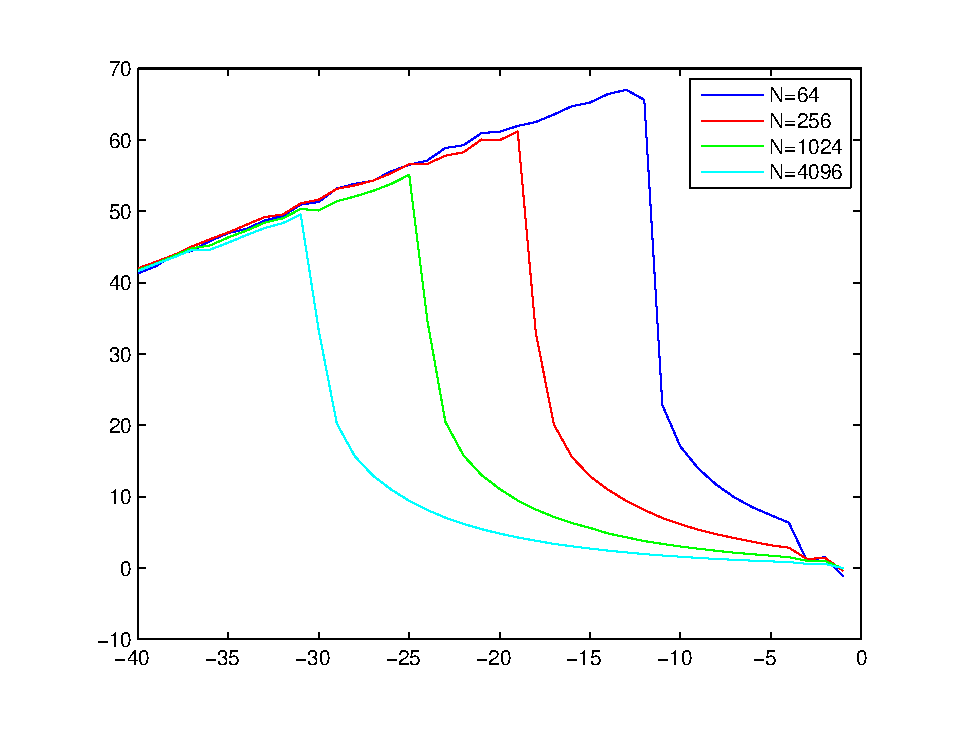
\includegraphics{test0.eps}
\end{figure}
\begin{figure}[H]
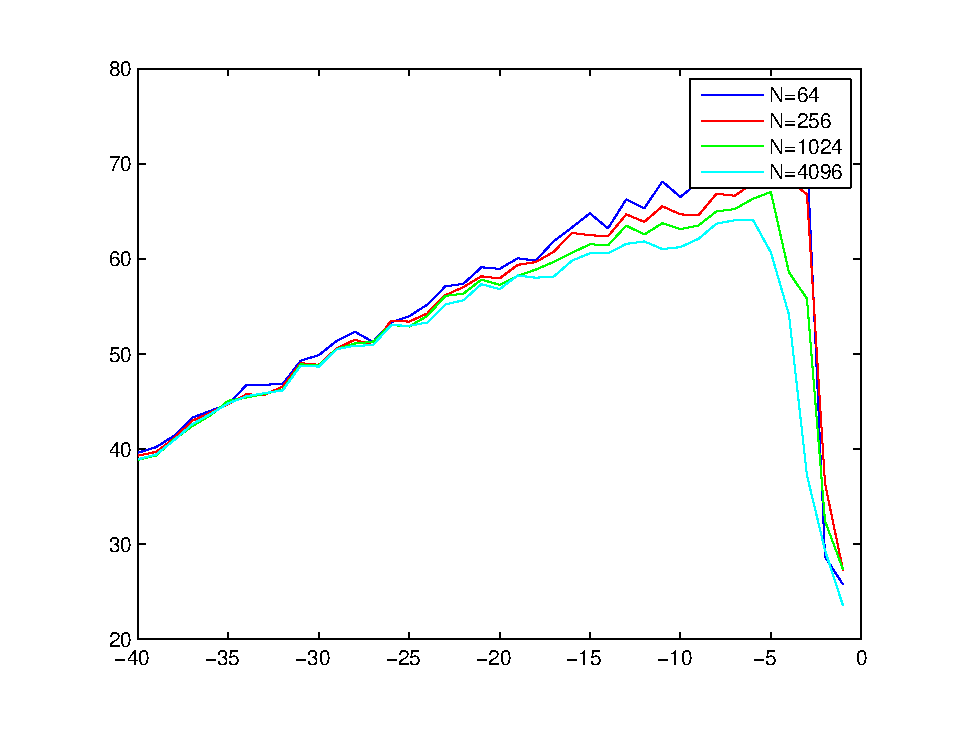
\includegraphics{test1.eps}
\end{figure}
\begin{figure}[H]
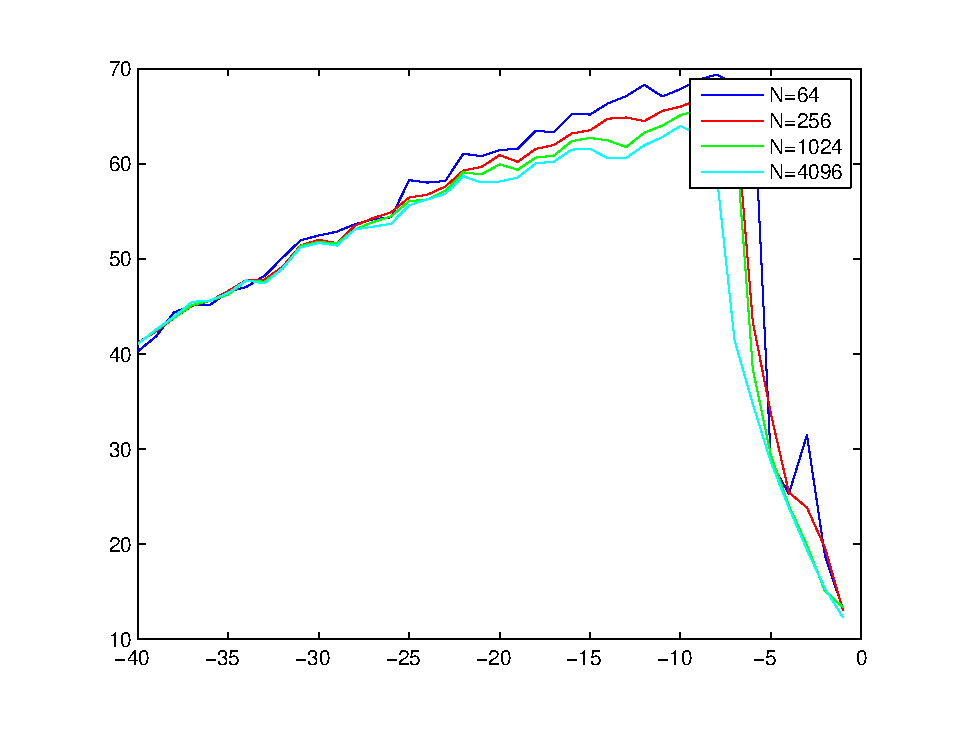
\includegraphics{test2.eps}
\end{figure}

\newpage

\section{fft.c}
\begin{lstlisting}

#include <stdio.h>
#include <stdlib.h>
#include <math.h>
#include <sys/time.h>

#include "complex.h"

#define PI 3.14159265359
#define MAXPOW 24

extern void set_taus_seed();

double gaussdouble(double,double);
unsigned int taus();
void randominit();

int pow_2[MAXPOW];
int pow_4[MAXPOW];

void twiddle(struct complex *W, int N, double stuff)
{
  W->r=cos(stuff*2.0*PI/(double)N);
  W->i=-sin(stuff*2.0*PI/(double)N);
}


void bit_r4_reorder(struct complex *W,// Final output  
		    int N)            // size of FFT

{
  int bits, i, j, k;
  double tempr, tempi;
    
  for (i=0; i<MAXPOW; i++)
    if (pow_2[i]==N) bits=i;

  for (i=0; i<N; i++)
    {
      j=0;
      for (k=0; k<bits; k+=2)
	{
	  if (i&pow_2[k]) j+=pow_2[bits-k-2];
	  if (i&pow_2[k+1]) j+=pow_2[bits-k-1];
	}

      if (j>i)  /** Only make "up" swaps */
	{
	  tempr=W[i].r;
	  tempi=W[i].i;
	  W[i].r=W[j].r;
	  W[i].i=W[j].i;
	  W[j].r=tempr;
	  W[j].i=tempi;
	}
    }
}

void twiddle_fixed(struct complex16 *W, int N, double stuff)
{
  W->r=(short)(32767.0*cos(stuff*2.0*PI/(double)N));
  W->i=(short)(-32767.0*sin(stuff*2.0*PI/(double)N));
}

void twiddle_fixed_Q17(struct complex32 *W, int N, double stuff)
{
  W->r=(int)(((1<<17)-1)*cos(stuff*2.0*PI/(double)N));
  W->i=(int)((1-(1<<17))*sin(stuff*2.0*PI/(double)N));
}

void bit_r4_reorder_fixed_Q15(struct complex16 *W, 
			      int N,
			      char scale)       // shift for output
{
  int bits, i, j, k;
  short tempr, tempi;
    
  for (i=0; i<MAXPOW; i++)
    if (pow_2[i]==N) bits=i;

  for (i=0; i<N; i++)
    {
      j=0;
      for (k=0; k<bits; k+=2)
	{
	  if (i&pow_2[k]) j+=pow_2[bits-k-2];
	  if (i&pow_2[k+1]) j+=pow_2[bits-k-1];
	}

      if (j>i)  /** Only make "up" swaps */
	{
	  tempr=W[i].r>>scale;
	  tempi=W[i].i>>scale;
	  W[i].r=W[j].r>>scale;
	  W[i].i=W[j].i>>scale;
	  W[j].r=tempr;
	  W[j].i=tempi;
	}
    }
}

void bit_r4_reorder_fixed_Q17(struct complex32 *W, int N)
{
  int bits, i, j, k;
  short tempr, tempi;
    
  for (i=0; i<MAXPOW; i++)
    if (pow_2[i]==N) bits=i;

  for (i=0; i<N; i++)
    {
      j=0;
      for (k=0; k<bits; k+=2)
	{
	  if (i&pow_2[k]) j+=pow_2[bits-k-2];
	  if (i&pow_2[k+1]) j+=pow_2[bits-k-1];
	}

      if (j>i)  /** Only make "up" swaps */
	{
	  tempr=W[i].r;
	  tempi=W[i].i;
	  W[i].r=W[j].r;
	  W[i].i=W[j].i;
	  W[j].r=tempr;
	  W[j].i=tempi;
	}
    }
}

/** RADIX-4 FFT ALGORITHM */
/* Double precision*/
void radix4(struct complex *x, int N)
{ 
  int    n2, k1, N1, N2;
  struct complex W, bfly[4];

  N1=4;
  N2=N/4;
    
  /** Do 4 Point DFT */ 
  for (n2=0; n2<N2; n2++)
    {
      /** Radix 4 butterfly */
      bfly[0].r = (x[n2].r + x[N2 + n2].r + x[2*N2+n2].r + x[3*N2+n2].r);
      bfly[0].i = (x[n2].i + x[N2 + n2].i + x[2*N2+n2].i + x[3*N2+n2].i);

      bfly[1].r = (x[n2].r + x[N2 + n2].i - x[2*N2+n2].r - x[3*N2+n2].i);
      bfly[1].i = (x[n2].i - x[N2 + n2].r - x[2*N2+n2].i + x[3*N2+n2].r);

      bfly[2].r = (x[n2].r - x[N2 + n2].r + x[2*N2+n2].r - x[3*N2+n2].r);
      bfly[2].i = (x[n2].i - x[N2 + n2].i + x[2*N2+n2].i - x[3*N2+n2].i);

      bfly[3].r = (x[n2].r - x[N2 + n2].i - x[2*N2+n2].r + x[3*N2+n2].i);
      bfly[3].i = (x[n2].i + x[N2 + n2].r - x[2*N2+n2].i - x[3*N2+n2].r);


      /** In-place results */
      for (k1=0; k1<N1; k1++)
	{
	  twiddle(&W, N, (double)k1*(double)n2);
	  x[n2 + N2*k1].r = bfly[k1].r*W.r - bfly[k1].i*W.i;
	  x[n2 + N2*k1].i = bfly[k1].i*W.r + bfly[k1].r*W.i;
	}
    }
    
  /** Don't recurse if we're down to one butterfly */
  if (N2!=1)
    for (k1=0; k1<N1; k1++)
      {
	radix4(&x[N2*k1], N2);
      }
}



/** RADIX-4 Fixed-point Normalized FFT ALGORITHM for Q15 arithmetic*/
/* To be filled in by you .... */

void radix4_fixed_Q15(struct complex16 *x,   // Input in Q15 forma

		      int N,                 // Size of FFT
		      unsigned char *scale,  // Pointer to scaling schedule
		      unsigned char stage )  // Stage of fft
                                             
{ 
  int    n2, k1, N1, N2;
  struct complex16 W, bfly[4];

  N1=4;
  N2=N/4;
    


  // Do 4 Point DFT  
  for (n2=0; n2<N2; n2++)
    {

      // scale Butterfly input
      x[n2].r          >>= scale[stage];
      x[N2+n2].r       >>= scale[stage];
      x[(2*N2) + n2].r >>= scale[stage];
      x[(3*N2) + n2].r >>= scale[stage];
      x[n2].i          >>= scale[stage];
      x[N2+n2].i       >>= scale[stage];
      x[(2*N2) + n2].i >>= scale[stage];
      x[(3*N2) + n2].i >>= scale[stage];
      
      // Radix 4 Butterfly

      bfly[0].r = SAT_ADD16( SAT_ADD16(x[n2].r,x[N2 + n2].r) , SAT_ADD16 (x[2*N2+n2].r ,  x[3*N2+n2].r));
      bfly[0].i = SAT_ADD16( SAT_ADD16(x[n2].i,x[N2 + n2].i) , SAT_ADD16 (x[2*N2+n2].i ,  x[3*N2+n2].i));

      bfly[1].r =  SAT_ADD16( SAT_ADD16(x[n2].r , x[N2 + n2].i ), - SAT_ADD16( x[2*N2+n2].r , x[3*N2+n2].i));
      bfly[1].i = SAT_ADD16 (SAT_ADD16(x[n2].i , -x[N2 + n2].r) , SAT_ADD16(-x[2*N2+n2].i , x[3*N2+n2].r));

      bfly[2].r = SAT_ADD16(SAT_ADD16(x[n2].r , -x[N2 + n2].r) , SAT_ADD16( x[2*N2+n2].r , -x[3*N2+n2].r));
      bfly[2].i = SAT_ADD16(SAT_ADD16(x[n2].i , -x[N2 + n2].i) , SAT_ADD16( x[2*N2+n2].i , -x[3*N2+n2].i));

      bfly[3].r = SAT_ADD16(SAT_ADD16(x[n2].r ,- x[N2 + n2].i) ,SAT_ADD16(-x[2*N2+n2].r , x[3*N2+n2].i));
	  bfly[3].i=SAT_ADD16(SAT_ADD16(x[n2].i,x[N2 + n2].r ),-SAT_ADD16(x[2*N2+n2].i ,  x[3*N2+n2].r));
 


      // In-place results
      for (k1=0; k1<N1; k1++)
		{
	  		twiddle_fixed(&W, N, (double)k1*(double)n2);
		    x[n2 + N2*k1].r = SAT_ADD16(FIX_MPY(bfly[k1].r,W.r) , -FIX_MPY( bfly[k1].i,W.i));
            x[n2 + N2*k1].i = SAT_ADD16(FIX_MPY(bfly[k1].i,W.r) , FIX_MPY(bfly[k1].r,W.i));
		}
    }
    
    // Don't recurse if we're down to one butterfly 
  if (N2!=1)
    for (k1=0; k1<N1; k1++)
      {
		radix4_fixed_Q15(&x[N2*k1], N2,scale,stage+1);
      }
}


/** RADIX-4 Fixed-point Normalized FFT ALGORITHM for Q15 arithmetic*/
/* To be filled in by you*/

void radix4_fixed_Q24xQ17(struct complex32 *x,   // Input in Q24 format 
			  int N,                 // Size of FFT
			  unsigned char *scale,  // Pointer to scaling schedule
			  unsigned char stage)   // Stage of fft
{ 
  int    n2, k1, N1, N2;
  struct complex32 W, bfly[4];

  N1=4;
  N2=N/4;
    


  // Do 4 Point DFT  
  for (n2=0; n2<N2; n2++)
    {

      // scale Butterfly input
      x[n2].r          >>= scale[stage];
      x[N2+n2].r       >>= scale[stage];
      x[(2*N2) + n2].r >>= scale[stage];
      x[(3*N2) + n2].r >>= scale[stage];
      x[n2].i          >>= scale[stage];
      x[N2+n2].i       >>= scale[stage];
      x[(2*N2) + n2].i >>= scale[stage];
      x[(3*N2) + n2].i >>= scale[stage];
      
      // Radix 4 Butterfly 
      bfly[0].r = SAT_ADD25( SAT_ADD25(x[n2].r,x[N2 + n2].r) , SAT_ADD25 (x[2*N2+n2].r ,  x[3*N2+n2].r));
      bfly[0].i = SAT_ADD25( SAT_ADD25(x[n2].i,x[N2 + n2].i) , SAT_ADD25 (x[2*N2+n2].i ,  x[3*N2+n2].i));

      bfly[1].r =  SAT_ADD25( SAT_ADD25(x[n2].r , x[N2 + n2].i) , - SAT_ADD25( x[2*N2+n2].r , x[3*N2+n2].i));
      bfly[1].i = SAT_ADD25 (SAT_ADD25(x[n2].i , -x[N2 + n2].r) , SAT_ADD25(-x[2*N2+n2].i , x[3*N2+n2].r));

      bfly[2].r = SAT_ADD25(SAT_ADD25(x[n2].r , -x[N2 + n2].r) , SAT_ADD25( x[2*N2+n2].r , -x[3*N2+n2].r));
      bfly[2].i = SAT_ADD25(SAT_ADD25(x[n2].i , -x[N2 + n2].i) , SAT_ADD25( x[2*N2+n2].i , -x[3*N2+n2].i));

      bfly[3].r = SAT_ADD25(SAT_ADD25(x[n2].r ,- x[N2 + n2].i) ,- SAT_ADD25(-x[2*N2+n2].r , x[3*N2+n2].i));
      bfly[3].i = SAT_ADD25(SAT_ADD25(x[n2].i , x[N2 + n2].r ), -SAT_ADD25(x[2*N2+n2].i ,  x[3*N2+n2].r));


      // In-place results
      for (k1=0; k1<N1; k1++)
	{
	  twiddle_fixed_Q17(&W, N, (double)k1*(double)n2);
	  x[n2 + N2*k1].r = SAT_ADD25(FIX_MPY25by18(bfly[k1].r,W.r) , -FIX_MPY25by18( bfly[k1].i,W.i));
      x[n2 + N2*k1].i = SAT_ADD25(FIX_MPY25by18(bfly[k1].i,W.r) , FIX_MPY25by18(bfly[k1].r,W.i));
	}
    }
    
    // Don't recurse if we're down to one butterfly 
  if (N2!=1)
    for (k1=0; k1<N1; k1++)
      {
	radix4_fixed_Q24xQ17(&x[N2*k1], N2,scale,stage+1);
      }
}


QAM_input(struct complex *data,double amp,int N,int Nu,char M) {

  int i,rv;
  int FCO = (N-(Nu>>1));   // First non-zero carrier offset

  for (i=0;i<N;i++) {
    data[i].r = 0.0;
    data[i].i = 0.0;
  }

  for (i=0;i<Nu;i++) {

    rv = taus();

    switch (M) {

    case 0 :   // QPSK
      data[(i+FCO)%N].r = ((rv&1) ? -amp : amp)/sqrt(2.0);
      data[(i+FCO)%N].r = (((rv>>1)&1) ? -amp : amp)/sqrt(2.0);
      break;
    case 1 :   // 16QAM 
      data[(i+FCO)%N].r = (2*(rv&3) - 3)*amp/sqrt(10);
      data[(i+FCO)%N].i = (2*((rv>>2)&3) - 3)*amp/sqrt(10);
      break;
    default:
      break;
    }
    
  }
}

void fft_distortion_test(int N,                              // dimension of FFT under test 
			 char test,                          // type of test
			 double input_dB,                    // strength of input
			 char *scale,                        // pointr to scaling schedule
			 double *maxSNR,                     // pointer best signal-to-noise ratio
			 char *maxscale,                     // pointer to best scaling schedule
			 struct complex *data,               // pointer to floating point data vector
			 struct complex16 *data16,           // pointer to Q15 data vector
			 struct complex32 *data32)           // pointer to Q17 data vector
{


  double mean_in=0.0,mean_error=0.0,SNR;
  int i;


  for (i=0; i<N; i++)
    {
      data[i].r=0.0;
      data[i].i=0.0;
      data16[i].r=0;
      data16[i].i=0;
      data32[i].r=0;
      data32[i].i=0;
	  
    }
      
      

  switch (test) {
  case 0:       /** Generate cosine **/
    for (i=0; i<N; i++)
      data[i].r=pow(10,.05*input_dB)*cos(2.0*PI*.1*i)*sqrt(2);

    break;
  case 1:    // QPSK
    QAM_input(data,pow(10,.05*input_dB),N,N,0);
    break;

  case 2:    // 16-QAM
    QAM_input(data,pow(10,.05*input_dB),N,N,1);
    break;

  default:
    break;
  }

  // Make fixed-point versions of data
  for (i=0;i<N;i++) {
    data16[i].r = (short)(data[i].r*32767);
    data16[i].i = (short)(data[i].i*32767);
    data32[i].r = (int)(data[i].r*32767);
    data32[i].i = (int)(data[i].i*32767);

  }

  // Do Floating-point FFT
  radix4(data, N);
  for (i=0;i<N;i++) {

    data[i].r /= sqrt(N);
    data[i].i /= sqrt(N);
  }
  bit_r4_reorder(data, N);

  // Do Q15 FFT
  radix4_fixed_Q15(data16, N,scale,0);
  bit_r4_reorder_fixed_Q15(data16, N,scale[6]);
		  

  // Compute Distortion statistics
  mean_error = 0.0;
  mean_in = 0.0;
  for (i=0;i<N;i++) {
    mean_in += data[i].r*data[i].r + data[i].i*data[i].i;
    mean_error += pow((data[i].r-((double)data16[i].r/32767.0)),2) + pow((data[i].i-((double)data16[i].i/32767.0)),2);
  }
		  
  SNR = 10*log10(mean_in/mean_error);
  // printf("%d %d %d %d %d %d %d : %f\n",scale[0],scale[1],scale[2],scale[3],scale[4],scale[5],scale[6],SNR);
  if (SNR > *maxSNR) {
    *maxSNR = SNR;
    memcpy(maxscale,scale,7);
  }



}

#define SCALE64 0x0006
#define SCALE256 0x0016
#define SCALE1024 0x0056
#define SCALE4096 0x0156

void main(int argc, char *argv[])
{

  int    N, radix=4,test;
  int    i;
  char scale[7],maxscale[7],MAXSHIFT;
  double maxSNR,input_dB;
  struct complex *data;
  struct complex16 *data16;  
  struct complex32 *data32;

  randominit();
  set_taus_seed();

  if (argc!= 3) {
    printf("fft size(16-4096) test(0-2)!!\n");
    exit(-1);
  }

  N = atoi(argv[1]);

  test = atoi(argv[2]);

  if ((N&1) == 1) {
    printf("Size must be a power of 4!\n");
    exit(-1);
  }
   
  if ((test>2) || (test<0)) {
    printf("test must be in (0-2)\n");
    exit(-1);
  }

  /** Set up power of two arrays */
  pow_2[0]=1;
  for (i=1; i<MAXPOW; i++)
    pow_2[i]=pow_2[i-1]*2;
  pow_4[0]=1;
  for (i=1; i<MAXPOW; i++)
    pow_4[i]=pow_4[i-1]*4;
    
  if ((data=malloc(sizeof(struct complex)*(size_t)N))==NULL)
    {
      fprintf(stderr, "Out of memory!\n");
      exit(1);
    }

  if ((data16=malloc(sizeof(struct complex16)*(size_t)N))==NULL)
    {
      fprintf(stderr, "Out of memory!\n");
      exit(1);
    }

  if ((data32=malloc(sizeof(struct complex32)*(size_t)N))==NULL)
    {
      fprintf(stderr, "Out of memory!\n");
      exit(1);
    }

  printf("res_%d = [ \n",N);    
  FILE *f1 = fopen("file64_2.txt", "w");
  if (f1==NULL){
		printf("Error opening file");
	    exit(1);


	}


FILE *f2 = fopen("file256_2.txt", "w");
  if (f2==NULL){
        printf("Error opening file");
        exit(1);


    }
FILE *f3 = fopen("file1024_2.txt", "w");
  if (f3==NULL){
        printf("Error opening file");
        exit(1);


    }
FILE *f4 = fopen("file4096_2.txt", "w");
  if (f4==NULL){
        printf("Error opening file");
        exit(1);


    }




  for (input_dB=-40;input_dB<0;input_dB++) {
    

    switch (N) {
    case 64:
      //  scale = SCALE64;
      MAXSHIFT=3;
      break;
    case 256:
      //      scale = SCALE256;
      MAXSHIFT=4;
      break;
    case 1024:
      //      scale = SCALE1024;
      MAXSHIFT=5;
      break;
    case 4096:
      //      scale = SCALE4096;
      MAXSHIFT=6;
      break;
    }

    for (i=0;i<7;i++)
      scale[i] = 0;

    maxSNR = -1000;
    switch (N) {
    case 4096:

      for (scale[0]=0;scale[0]<=MAXSHIFT;scale[0]++)
	for (scale[1]=0;scale[1]<=MAXSHIFT-scale[0];scale[1]++)
	  for (scale[2]=0;scale[2]<=MAXSHIFT-scale[0]-scale[1];scale[2]++)
	    for (scale[3]=0;scale[3]<=MAXSHIFT-scale[0]-scale[1]-scale[2];scale[3]++)
	      for (scale[4]=0;scale[4]<=MAXSHIFT-scale[0]-scale[1]-scale[2]-scale[3];scale[4]++)
		for (scale[5]=0;scale[5]<=MAXSHIFT-scale[0]-scale[1]-scale[2]-scale[3]-scale[4];scale[5]++){
		  scale[6]=MAXSHIFT-scale[0]-scale[1]-scale[2]-scale[3]-scale[4]-scale[5];
		  fft_distortion_test(N,test,input_dB,scale,&maxSNR,maxscale,data,data16,data32);
		
	      }
      printf("%f, %f, %% Optimum Scaling : %d %d %d %d %d %d %d\n",input_dB,maxSNR,maxscale[0],maxscale[1],maxscale[2],maxscale[3],maxscale[4],maxscale[5],maxscale[6]);
	  fprintf(f4, "%f, %f\n", input_dB, maxSNR);
      break;
    case 1024:

      for (scale[0]=0;scale[0]<=MAXSHIFT;scale[0]++)
	for (scale[1]=0;scale[1]<=MAXSHIFT-scale[0];scale[1]++)
	  for (scale[2]=0;scale[2]<=MAXSHIFT-scale[0]-scale[1];scale[2]++)
	    for (scale[3]=0;scale[3]<=MAXSHIFT-scale[0]-scale[1]-scale[2];scale[3]++) 
	      for (scale[4]=0;scale[4]<=MAXSHIFT-scale[0]-scale[1]-scale[2]-scale[3];scale[4]++){
		scale[6]=MAXSHIFT-scale[0]-scale[1]-scale[2]-scale[3]-scale[4];
		fft_distortion_test(N,test,input_dB,scale,&maxSNR,maxscale,data,data16,data32);
	      }
      printf("%f, %f, %% Optimum Scaling : %d %d %d %d %d %d %d\n",input_dB,maxSNR,maxscale[0],maxscale[1],maxscale[2],maxscale[3],maxscale[4],maxscale[5],maxscale[6]);
      fprintf(f3, "%f, %f\n", input_dB, maxSNR);
      break;
    case 256:

      for (scale[0]=0;scale[0]<=MAXSHIFT;scale[0]++)
	for (scale[1]=0;scale[1]<=MAXSHIFT-scale[0];scale[1]++)
	  for (scale[2]=0;scale[2]<=MAXSHIFT-scale[0]-scale[1];scale[2]++)
	    for (scale[3]=0;scale[3]<=MAXSHIFT-scale[0]-scale[1]-scale[2];scale[3]++) {
	      scale[6]=MAXSHIFT-scale[0]-scale[1]-scale[2]-scale[3];
	      fft_distortion_test(N,test,input_dB,scale,&maxSNR,maxscale,data,data16,data32);
	  }
      printf("%f, %f, %% Optimum Scaling : %d %d %d %d %d %d %d\n",input_dB,maxSNR,maxscale[0],maxscale[1],maxscale[2],maxscale[3],maxscale[4],maxscale[5],maxscale[6]);
      
	fprintf(f2, "%f, %f\n", input_dB, maxSNR);
	break;

    case 64:

      for (scale[0]=0;scale[0]<=MAXSHIFT;scale[0]++)
	for (scale[1]=0;scale[1]<=MAXSHIFT-scale[0];scale[1]++)
	  for (scale[2]=0;scale[2]<=MAXSHIFT-scale[0]-scale[1];scale[2]++) {
	      scale[6]=MAXSHIFT-scale[0]-scale[1]-scale[2];
	      fft_distortion_test(N,test,input_dB,scale,&maxSNR,maxscale,data,data16,data32);
	  }
      printf("%f, %f, %% Optimum Scaling : %d %d %d %d %d %d %d\n",input_dB,maxSNR,maxscale[0],maxscale[1],maxscale[2],maxscale[3],maxscale[4],maxscale[5],maxscale[6]);
	  fprintf(f1, "%f, %f\n", input_dB, maxSNR);
      break;

    }
  }
fclose(f1);
fclose(f2);
fclose(f3);
fclose(f4);
}

\end{lstlisting}





\end{document}

